% !TeX encoding = UTF-8
% !TeX spellcheck = LaTeX
% !TeX program = XeLaTeX
%

% Please compile by 'xelatex -shell-escape pre.tex' 

\documentclass[UTF-8]{beamer}

\usepackage{graphicx}
\usepackage{tikz}
\usepackage{amsmath,amssymb}
\usepackage{bm}
\usepackage{extarrows}
\usepackage{newtxtext}
\usepackage{minted}
\undef\checkmark
\usepackage{dingbat}
\usepackage{listings}
\usepackage{caption}
\usepackage{xcolor}

\usetheme{CambridgeUS}
\usecolortheme{crane}
\usefonttheme{professionalfonts}
\setbeamertemplate{footjoline}[frame number]
\useoutertheme{infolines}

\definecolor{bg}{rgb}{0.95,0.95,0.95}
\renewcommand{\listingscaption}[1]{\begin{center}CODE: #1\end{center}\vspace{-20pt}}
\setminted{
    fontsize=\small, 
    bgcolor=bg, frame=lines,
    mathescape, breaklines, breakanywhere,
    breaksymbolleft=\raisebox{0.8ex}{\small\reflectbox{\carriagereturn}},
    breaksymbolright=\small\carriagereturn
}

\setbeamercolor{thxcolor}{fg=white,bg=darkred}

\usetikzlibrary{shapes.geometric, arrows}
\tikzstyle{startstop} = [rectangle, rounded corners, minimum width=2.5cm, minimum height=1cm, text centered, 
draw=black, fill=red!30, font=\bf]
\tikzstyle{io} = [trapezium, trapezium left angle=70, trapezium right angle=110, minimum width=2.5cm, minimum height=1cm,
text centered, draw=black, fill=blue!30, font=\bf]
\tikzstyle{process} = [rectangle, minimum width=2.5cm, minimum height=1cm, text centered, 
draw=black, fill=orange!30, font=\bf]
\tikzstyle{decision} = [diamond, minimum width=2.5cm, minimum height=1cm, text centered, 
draw=black, fill=green!30, font=\bf]
\tikzstyle{arrow} = [thick, ->, >= stealth]
\tikzstyle{line} = [thick]

\title{MiniProver}
\subtitle{A coq-like proof assistant}
\institute{Peking University}
\author{Zhenwen Li, Sirui Lu, Kewen Wu}
\date{\today}

\begin{document}
\frame{\titlepage}

\begin{frame}{Accomplishment}
\begin{itemize}
\item Encode the dependent lambda calculus. 
\item Inductive types and induction rules.
\item Fix point operator and termination checking.
\item Dependent pattern matching.
\item Tactic-based proving and proof object reconstruction.
\item Formalize some interesting proofs in our system.
\end{itemize}
\end{frame}

\section{Type System}
\subsection{Calculus of Inductive Constructions}
\begin{frame}{$\lambda$-cube}
    \centering
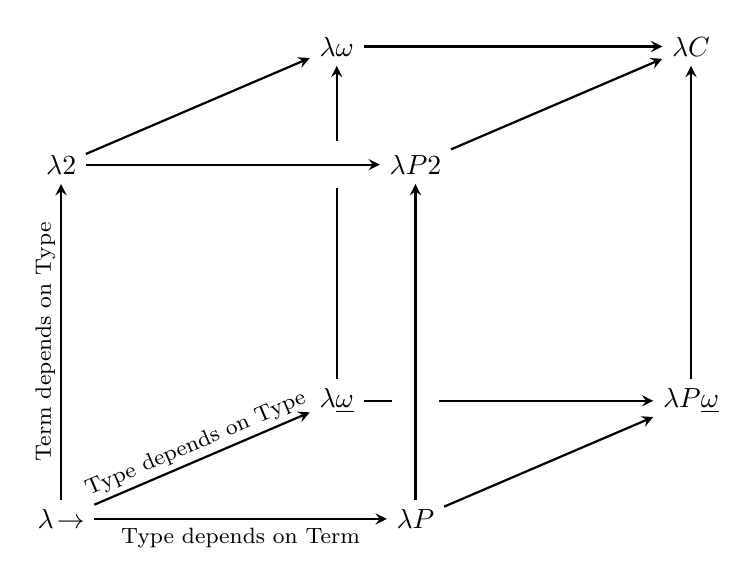
\begin{tikzpicture}[node distance=4.5cm]
    \node (la) {$\lambda\!\to$};
    \node (l2) [above of=la] {$\lambda 2$};
    \node (lp) [right of=la] {$\lambda P$};
    \node (lw') [right of=la, xshift=-1cm, yshift=1.5cm] {$\lambda \underline{\omega}$};
    \node (lw) [above of=lw'] {$\lambda \omega$};
    \node (lc) [right of=lw] {$\lambda C$};
    \node (lpw) [right of=lw'] {$\lambda P\underline{\omega}$};
    \node (lp2) [above of=lp] {$\lambda P2$};

    \footnotesize
        
    \path[->, thick, >=stealth] (lw') edge (lw) edge (lpw);
    \node[fill=white, minimum size=6mm] at (3.5,4.5) {};
    \node[fill=white, minimum size=6mm] at (4.5,1.5) {};
    \path[->, thick, >=stealth] 
        (la) edge node[below] {Type depends on Term} (lp)  
            edge node[sloped,yshift=2mm] {Term depends on Type} (l2)
            edge node[sloped,yshift=2mm] {Type depends on Type} (lw')
        (lp) edge (lpw) edge (lp2)
        (l2) edge (lp2) edge (lw)
        (lw) edge (lc)
        (lp2) edge (lc)
        (lpw) edge (lc);
\end{tikzpicture}
\end{frame}

\begin{frame}{Example and \textbf{CIC}}
\begin{itemize}
\item Term depends on Type\\
    $\tt\lambda T:Type.\ \lambda x:T.\ x\quad :\quad \Pi T:Type.\ T\to T$
\item Type depends on Type\\
    $\tt\lambda T:Type.\ T\to T\quad :\quad Type\to Type$
\item Type depends on Term\\
    $\tt\lambda n:nat.\ S\ n\quad :\quad nat\to Type$
        \vspace{10pt}
\item $\lambda C$ + \textit{Definition} $\Rightarrow$ $\lambda D$.\\
\item $\lambda D$ + \textit{Inductive Type} $\Rightarrow$ \textbf{CIC}.
\end{itemize}
\end{frame}

\subsection{Key Typing Rule}
\begin{frame}[fragile]{Inductive Type}
$$
\tt Ind\ [{\it p}]\ (\Gamma_I:=\Gamma_C)
$$
\vspace{-10pt}
\begin{itemize}
\item $\it p$ : Number of parameters.
\item $\tt \Gamma_I$ : Inductive type.
\item $\tt \Gamma_C$ : Constructors of the inductive type.
\end{itemize}
\vspace{10pt}
\begin{minted}{coq}
Inductive lst (T : Type) : Type :=
    | nil : lst T
    | cons : T -> lst T -> lst T
\end{minted}
$$
\small
\tt Ind\ [1]\left([lst:Type\to Type]:=
\begin{bmatrix}
\tt nil:\Pi T:Type,\ lst\ T\\
\tt cons:\Pi T:Type,\ T\to lst\ T\to lst\ T
\end{bmatrix}\right)
$$
\end{frame}

\begin{frame}[fragile]{Match}
$$\tt match\ {\it t}\ as\ {\it x_0}\ in\ {\it namelist}\ return\ {\it returntype}\ with\ [{\it equation}]$$
\begin{itemize}
    \item $\it t$ : A term of inductive type.
    \item $\it namelist$ : Arguments of the inductive type.
    \item $\it equation$ : Different constructors of the inductive type.
\end{itemize}

\begin{minted}{coq}
Inductive eq (T : Type) (x : T) : T -> Type :=
    | eq_refl : eq T x x

fun (n : nat) (m : nat) (e : eq nat n m) =>
    match e in (eq _ _ y) return (eq nat y n) with
    | eq_refl _ _ => ...
\end{minted}
\end{frame}

\subsection{Termination}
\begin{frame}[fragile]{Termination Check}
\begin{minted}[escapeinside=<>]{coq}
Fixpoint plus (<\colorbox{green}{n}> m : nat) : nat :=
    match <\colorbox{green}{n}> with
    | O => m
    | S p => S (plus <\colorbox{green}{p}> m)

Fixpoint plus' (<\colorbox{green}{n}> <\colorbox{red}{m}> : nat) : nat :=
    match <\colorbox{green}{n}> with
    | O => m
    | S p => S (plus <\colorbox{red}{m}> <\colorbox{green}{p}>)
\end{minted}
\begin{alertblock}{Criterion}
    Descending on at least one variable.
\end{alertblock}
\end{frame}

\subsection{Inductive Positivity}
\begin{frame}[fragile]{Positivity Check}
\begin{minted}[escapeinside=<>]{coq}
Inductive ill : Type :=
    | malf : (ill -> ill) -> ill 

Definition extract (t : ill) : ill :=
    match t with
    | malf f => f t

    extract (malf extract)  (* not terminating *)
\end{minted}
\begin{alertblock}{Criterion}
    Types of constructors satisfy \textbf{positivity condition} for name of inductive type.
\end{alertblock}
\end{frame}

\section{Top Level}
\begin{frame}[fragile]{Build Term and Type for Inductive Definition}
\begin{exampleblock}{Intuition}
    View mathematical induction as building a term for inductive definition.
\end{exampleblock}

\begin{minted}[escapeinside=<>]{coq}
Inductive nat : Type := O : nat | S : nat -> nat

fun (P : nat -> Type) (f : P O) 
        (f0 : forall n : nat, P n -> P (S n)) 
    fix F (n : nat) : P n :=
        match n as n0 in (nat) return (P n0) with
        | O => f
        | S n0 => f0 n0 (F n0)
:
forall P : nat -> Type, P O -> 
    (forall n : nat, P n -> P (S n)) -> 
        forall n: nat, P n
\end{minted}
\end{frame}

\section{Evaluation}
\begin{frame}{Evaluation (Conversion)}
\begin{itemize}
    \item $\beta$-reduction : Reduce \textit{application}
    \item $\iota$-reduction : Reduce {\tt match}
    \item $\delta$-reduction : $\tt Definition\ x\ :=\ u$ \quad $\Rightarrow$\quad $\tt x\to u$
    \item $\zeta$-reduction : $\tt let\ x\ :=\ u\ in\ t$ \quad $\Rightarrow$\quad $\tt [x\to u]t$
    \item $\eta$-expansion : $\tt t:\forall x:T,U$ \quad $\Rightarrow$\quad $\tt \lambda x:T.\ (t\ x)$
\end{itemize}
\end{frame}

\section{Proof Handling}
\begin{frame}{Proof Handling}
\begin{itemize}
\item Build proof object.
\item Navigate : Undo.
\item Switch mode : Proof, Qed, Abort.
\item Request info : Print.
\end{itemize}
\end{frame}

\section{Tactic}
\begin{frame}{Tactics}
\begin{itemize}
\item Intro, Intros : $\tt \vdash A\to B$ $\Rightarrow$ $\tt A\vdash B$
\item Apply : $\tt A\to B\vdash B$ $\Rightarrow$ $\tt A\to B\vdash A$
\item Exact : Construct the term manually
\item Reflexivity : $\tt eq\ T\ x\ y$ $\Rightarrow$ check if $\tt x=_{\beta\delta\iota\eta\zeta}y$
\item Split : $\tt \vdash P_1\wedge P_2$ $\Rightarrow$ $\tt \vdash P_1,P_2$
\item Induction : Classified sub-proofs with induction hypothesis
\item Equivalence : Build equivalence relations inside inductive term
\end{itemize}
\end{frame}

\begin{frame}{Tactics}
\begin{itemize}
\item Simpl : Simplify into human-readable goal 
\item Destruct : Classified sub-proofs without induction hypothesis
\item Left, Right : $\tt \vdash P_1\vee P_2$ $\Rightarrow$ $\tt \vdash P_1$ or $\tt\vdash P_2$ 
\item Symmetry : $\tt eq\ T\ x\ y\vdash eq\ T\ y\ x$
\item Rewrite : $\tt eq\ T\ x\ y$ $\Rightarrow$ $\tt x\to y$ or $\tt y\to x$
\item Unfold : Replace term with $\beta\iota$-normal form
\item Exists : $\tt \vdash\exists x,\ P\ x$ $\Rightarrow$ $\tt x_0\wedge(P\ x_0)$
\end{itemize}
\end{frame}

\section*{Thanks}
\begin{frame}
\LARGE
\begin{beamercolorbox}[center,ht=3em]{thxcolor}
\vspace{1em}
\Huge Thanks!
\end{beamercolorbox}
\end{frame}\end{document}
